%%%%%%%%%%%%%%%%%%%%%%%%%%%%%%%%%%%%%%%%%%%%%%%%%%%%%%%%%%%%%%%%%%%%%%%%%%%%%%%%%
%% Documenclass 
%%%%%%%%%%%%%%%%%%%%%%%%%%%%%%%%%%%%%%%%%%%%%%%%%%%%%%%%%%%%%%%%%%%%%%%%%%%%%%%%%
\documentclass[a4paper,oneside,titlepage]{report}
%%%%%%%%%%%%%%%%%%%%%%%%%%%%%%%%%%%%%%%%%%%%%%%%%%%%%%%%%%%%%%%%%%%%%%%%%%%%%%%%%
%% Packages
%%%%%%%%%%%%%%%%%%%%%%%%%%%%%%%%%%%%%%%%%%%%%%%%%%%%%%%%%%%%%%%%%%%%%%%%%%%%%%%%%
\usepackage[english]{babel}
\usepackage{amsmath}
\usepackage{complexity}
\usepackage[T1]{fontenc}
\usepackage[utf8]{inputenc}
\usepackage[pdftex]{graphicx} %%Graphics in pdfLaTeX
\usepackage{a4wide} %%Smaller margins, more text per page.
\usepackage{longtable} %%For tables that exceed a page width
\usepackage{pdflscape} %%Adds PDF sup­port to the land­scape en­vi­ron­ment of pack­age
\usepackage{caption} %%Pro­vides many ways to cus­tomise the cap­tions in float­ing en­vi­ron­ments like fig­ure and ta­ble
\usepackage{float} %%Im­proves the in­ter­face for defin­ing float­ing ob­jects such as fig­ures and ta­bles
\usepackage[tablegrid,nochapter]{vhistory} %%Vhis­tory sim­pli­fies the cre­ation of a his­tory of ver­sions of a doc­u­ment
\usepackage[nottoc]{tocbibind} %%Au­to­mat­i­cally adds the bib­li­og­ra­phy and/or the in­dex and/or the con­tents, etc., to the Ta­ble of Con­tents list­ing
\usepackage[toc,page]{appendix} %%The ap­pendix pack­age pro­vides var­i­ous ways of for­mat­ting the ti­tles of ap­pen­dices
\usepackage{pdfpages} %%This pack­age sim­pli­fies the in­clu­sion of ex­ter­nal multi-page PDF doc­u­ments in LATEX doc­u­ments
\usepackage[rightcaption]{sidecap} %%De­fines en­vi­ron­ments called SC­fig­ure and SCtable (anal­o­gous to fig­ure and ta­ble) to type­set cap­tions side­ways
\usepackage{cite} %%The pack­age sup­ports com­pressed, sorted lists of nu­mer­i­cal ci­ta­tions, and also deals with var­i­ous punc­tu­a­tion and other is­sues of rep­re­sen­ta­tion, in­clud­ing com­pre­hen­sive man­age­ment of break points
\usepackage[]{acronym} %%This pack­age en­sures that all acronyms used in the text are spelled out in full at least once. It also pro­vides an en­vi­ron­ment to build a list of acronyms used
\usepackage[pdftex,scale={.8,.8}]{geometry} %%The pack­age pro­vides an easy and flex­i­ble user in­ter­face to cus­tomize page lay­out, im­ple­ment­ing auto-cen­ter­ing and auto-bal­anc­ing mech­a­nisms so that the users have only to give the least de­scrip­tion for the page lay­out. For ex­am­ple, if you want to set each mar­gin 2cm with­out header space, what you need is just \usep­a­ck­age[mar­gin=2cm,no­head]{ge­om­e­try}.
\usepackage{layout} %%The pack­age de­fines a com­mand \lay­out, which will show a sum­mary of the lay­out of the cur­rent doc­u­ment
\usepackage{subfigure} %%Pro­vides sup­port for the ma­nip­u­la­tion and ref­er­ence of small or ‘sub’ fig­ures and ta­bles within a sin­gle fig­ure or ta­ble en­vi­ron­ment.
\usepackage[toc]{glossaries} %%The glos­saries pack­age sup­ports acronyms and mul­ti­ple glos­saries, and has pro­vi­sion for op­er­a­tion in sev­eral lan­guages (us­ing the fa­cil­i­ties of ei­ther ba­bel or poly­glos­sia).

\usepackage[left,pagewise,modulo]{lineno} %%Adds line num­bers to se­lected para­graphs with ref­er­ence pos­si­ble through the LATEX \ref and \pageref cross ref­er­ence mech­a­nism
\usepackage[pdftex,colorlinks=false,hidelinks,pdfstartview=FitV]{hyperref}%%The hy­per­ref pack­age is used to han­dle cross-ref­er­enc­ing com­mands in LATEX to pro­duce hy­per­text links in the doc­u­ment. 
\usepackage{metainfo}
\usepackage[pagestyles,raggedright]{titlesec}
\usepackage{etoolbox}
\usepackage{%
	array, %%An ex­tended im­ple­men­ta­tion of the ar­ray and tab­u­lar en­vi­ron­ments which ex­tends the op­tions for col­umn for­mats, and pro­vides "pro­grammable" for­mat spec­i­fi­ca­tions
	booktabs, %%The pack­age en­hances the qual­ity of ta­bles in LATEX, pro­vid­ing ex­tra com­mands as well as be­hind-the-scenes op­ti­mi­sa­tion
	dcolumn, %%
	rotating,
	shortvrb,
	units,
	url,
	lastpage,
	longtable,
	lscape,
	qtree,
	skmath,	
}
%%%%%%%%%%%%%%%%%%%%%%%%%%%%%%%%%%%%%%%%%%%%%%%%%%%%%%%%%%%%%%%%%%%%%%%%%%%%%%%%%
%% Java --> latex 
%%%%%%%%%%%%%%%%%%%%%%%%%%%%%%%%%%%%%%%%%%%%%%%%%%%%%%%%%%%%%%%%%%%%%%%%%%%%%%%%%
\usepackage{listings}
\usepackage{color}
\definecolor{pblue}{rgb}{0.13,0.13,1}
\definecolor{pgreen}{rgb}{0,0.5,0}
\definecolor{pred}{rgb}{0.9,0,0}
\definecolor{pgrey}{rgb}{0.46,0.45,0.48}
\usepackage{inconsolata}
%%Listing style for java.
\definecolor{dkgreen}{rgb}{0,0.6,0}
\definecolor{gray}{rgb}{0.5,0.5,0.5}
\definecolor{mauve}{rgb}{0.58,0,0.82}
\lstset{frame=tb,
	language=Java,
	aboveskip=3mm,
	belowskip=3mm,
	showstringspaces=false,
	columns=flexible,
	basicstyle={\small\ttfamily},
	numbers=left,
	numberstyle=\tiny\color{gray},
	keywordstyle=\color{blue},
	commentstyle=\color{dkgreen},
	stringstyle=\color{mauve},
	breaklines=true,
	breakatwhitespace=true,
	tabsize=3
}

%%%%%%%%%%%%%%%%%%%%%%%%%%%%%%%%%%%%%%%%%%%%%%%%%%%%%%%%%%%%%%%%%%%%%%%%%%%%%%%%%
\setlength{\parindent}{0pt}
\setlength{\parskip}{.5\baselineskip}
%%%%%%%%%%%%%%%%%%%%%%%%%%%%%%%%%%%%%%%%%%%%%%%%%%%%%%%%%%%%%%%%%%%%%%%%%%%%%%%%%
%% Inserting the metadata
%%%%%%%%%%%%%%%%%%%%%%%%%%%%%%%%%%%%%%%%%%%%%%%%%%%%%%%%%%%%%%%%%%%%%%%%%%%%%%%%%
\def\Institute{\textit{The University of Alabama}}
\def\Course{\textit{CS495}}

\def\BoldTitle{Software Requirements Specification}

\def\Subtitle{for \\ MEISR Application \\}
\def\Authors{Prepared by Kevin Ziegler, Chase Feaster, John Andrews, Stephen Bowles, Sung Kim}


\title{\textbf{\BoldTitle}\\\Subtitle}
\author{\Authors \\ \\ \\ \Institute\\ \Course\\}
\date{27 February 2018}

%%%%%%%%%%%%%%%%%%%%%%%%%%%%%%%%%%%%%%%%%%%%%%%%%%%%%%%%%%%%%%%%%%%%%%%%%%%%%%%%%
%% Creation of pdf information
%%%%%%%%%%%%%%%%%%%%%%%%%%%%%%%%%%%%%%%%%%%%%%%%%%%%%%%%%%%%%%%%%%%%%%%%%%%%%%%%%
\hypersetup{pdfinfo={
		Title={Title},
		Author={TR},
		Subject={Report}
	}}
%%%%%%%%%%%%%%%%%%%%%%%%%%%%%%%%%%%%%%%%%%%%%%%%%%%%%%%%%%%%%%%%%%%%%%%%%%%%%%%%%
%% Creating the frontpage
%%%%%%%%%%%%%%%%%%%%%%%%%%%%%%%%%%%%%%%%%%%%%%%%%%%%%%%%%%%%%%%%%%%%%%%%%%%%%%%%%
\AtBeginDocument{
	\maketitle
	\thispagestyle{empty}
}

%%%%%%%%%%%%%%%%%%%%%%%%%%%%%%%%%%%%%%%%%%%%%%%%%%%%%%%%%%%%%%%%%%%%%%%%%%%%%%%%%
%% Creation of the header
%%%%%%%%%%%%%%%%%%%%%%%%%%%%%%%%%%%%%%%%%%%%%%%%%%%%%%%%%%%%%%%%%%%%%%%%%%%%%%%%%
\patchcmd{\chapter}{plain}{short}{}{} %$ <-- the header on chapter 1
%%%%%%%%%%%%%%%%%%%%%%%%%%%%%%%%%%%%%%%%%%%%%%%%%%%%%%%%%%%%%%%%%%%%%%%%%%%%%%%%%
%% Creation of page-styles
%%%%%%%%%%%%%%%%%%%%%%%%%%%%%%%%%%%%%%%%%%%%%%%%%%%%%%%%%%%%%%%%%%%%%%%%%%%%%%%%%
\newpagestyle{long}{%
	\sethead[\thepage][][\chaptername\ \thechapter:\ \chaptertitle]{\chaptername\ \thechapter:\ \chaptertitle}{}{\thepage}
	\headrule
}

\newpagestyle{short}{%
	\sethead[\thepage][][]{}{}{\thepage}
	\headrule
}
% Make Glossary
%%%%%%%%%%%%%%%%%%%%%%%%%%%%%%%%%%%%%%%%%%%%%%%%%%%%%%%%%%%%%%%%%%%%%%%%%%%%%%%%%
%% DOCUMENT
%%%%%%%%%%%%%%%%%%%%%%%%%%%%%%%%%%%%%%%%%%%%%%%%%%%%%%%%%%%%%%%%%%%%%%%%%%%%%%%%%
\begin{document}

\pagenumbering{roman}
\DeclareGraphicsExtensions{.pdf,.jpg,.png}
\pagestyle{short}



\newpage
%%%%%%%%%%%%%%%%%%%%%%%%%%%%%%%%%%%%%%%%%%%%%%%%%%%%%%%%%%%%%%%%%%%%%%%%%%%%%%%%%
%% Table of contents
%%%%%%%%%%%%%%%%%%%%%%%%%%%%%%%%%%%%%%%%%%%%%%%%%%%%%%%%%%%%%%%%%%%%%%%%%%%%%%%%%
 \tableofcontents % Inhaltsverzeichnis



\pagestyle{long}




%%%%%%%%%%%%%%%%%%%%%%%%%%%%%%%%%%%%%%%%%%%%%%%%%%%%%%%%%%%%%%%%%%%%%%%%%%%%%%%%%
%% Version table insertion
%%%%%%%%%%%%%%%%%%%%%%%%%%%%%%%%%%%%%%%%%%%%%%%%%%%%%%%%%%%%%%%%%%%%%%%%%%%%%%%%%
% Versionstabelle.

\chapter*{Revision History}
\addcontentsline{toc}{chapter}{Revision History}
\begin{versionhistory}
	\vhEntry{1.0}{2/6/2018}{MEISR Team}{Introduction,Functional, Nonfunctional, Glossary, Features}
    \vhEntry{1.1}{2/8/2018}{MEISR Team}{Competitors, UML Diagrams}
    \vhEntry{1.2}{2/15/2018}{MEISR Team}{Formatting, UML Text Descriptions}
    \vhEntry{1.3}{2/22/2018}{John Andrews}{Add figure numbers}
    \vhEntry{2.1}{3/30/2018}{MEISR Team}{Sequence Diagrams, Database Schema, and Class Diagram}
    \vhEntry{2.2}{4/1/2018}{Sungkyun Kim}{Add diagram and database schema Text}
    \vhEntry{2.2}{4/1/2018}{John Andrews}{Add sequence diagram text}
    


\end{versionhistory}
\pagenumbering{arabic}
%%%%%%%%%%%%%%%%%%%%%%%%%%%%%%%%%%%%%%%%%%%%%%%%%%%%%%%%%%%%%%%%%%%%%%%%%%%%%%%%%
%% Inserting all the content
%%%%%%%%%%%%%%%%%%%%%%%%%%%%%%%%%%%%%%%%%%%%%%%%%%%%%%%%%%%%%%%%%%%%%%%%%%%%%%%%%
\chapter{Introduction \& Project Description}
\label{ch:intro}

\section{Preface}
MEISR is a profiling tool developed to measure and track a child’s general development in engagement, independence, and social engagement as they grow. The current MEISR tool is comprised of twenty-two pages of survey material culminating in a series of scoring calculations. The MEISR app for the Android platform, hence referred to as the MEISR App, is designed to simplify the process of completing, scoring, and evaluating the MEISR by presenting the survey in a simplified format, performing scoring calculations automatically, and presenting useful, graphical results for professional review.

\section{Features}
	
The website provides a login system for the data analyst with security features to protect the child’s information. (required)

The Android application intelligently decide how much of the survey the guardian needs to fill out. (required)
E.g. If a guardian fills in 3 “1s” in a row for a routine, then the algorithm will automatically go on to the next routine.
E.g. If a guardian has previous filled out 3’s for a routine, then the algorithm will not display those routines since it is clear the child has mastered those routines.

The Android application displays a graph summary of the score, which is calculated once the Guardian fills out the survey. (required)

Once a survey is scored the information is sent to a database. The website can be used to query this database to find trends or results (required)

The website also allows the guardian to fill out a survey and receive the results. The website would also follow the same algorithm for intelligently deciding how much of the survey the guardian needs to fill out. (possible)

Cross-platform functionality beyond just Android would be a goal that we could do if time was available. (future work if time available)




\chapter{Functional and Non-Functional Requirements}
\label{ch:Functional and Non-Functional Requirements}

\section{Functional Requirements}

The system can create a new account with information provided from the user.

The system can login a user to the system.

The user can start a new MEISR survey.

The user can continue a MEISR survey.

The user can save a MEISR survey.

The user can score a MEISR survey.

The user can export the results of a MEISR survey by printing or saving the file.

The user can logout.

The system sends the data generated from the scored reports to a database.

Administrative login.

The Administrator can query the database.

The Administrator can update the survey itself.

\section{Non-Functional Requirements}


Accessibility is very important. Therefore, the app needs to be computationally undemanding and viable with as many android versions as possible.

The user needs to be able to save and resume the survey at a later time, since it might not be possible for a person to complete the survey in one sitting.

Directions and scoring need to be intuitive making the survey easier to complete and score than the paper version.

Follow FERPA and HIPPA guidelines on access and storage of personal information.

Back-end database which can store survey results and allow researchers to analyze data.

Free access for users.


\newpage


\chapter{Competitors}
\label{ch:Competitors}
\section{The Child Development Tracking App Space}
The most relevant app in our market is the Center for Disease Control’s Milestone Tracker app. It is used to track your child development to see if they are lacking in certain areas. The other apps are the top similar/suggested results for the CDC Milestone Tracker app. These apps are not necessarily direct competitors to the MEISR app as they are designed to be more general, and only provide a simple checklist of common milestones. Our app specifically scores the development of a child based on the MEISR tool. However, these apps do have some features that could be worth looking into. Some features such as adding multiple children/social media are not applicable due to the fact that our app is intended for children with disabilities and privacy is a concern.

\section{Comparison of Features}
\begin{center}
\begin{tabular}{ c c c c c}
  & Age (months) & Charts & Scoring & Sharing \\
 CDC Milestone Tracker & 2-60 & no & no & no\\
 The Wonder Weeks App & 0-20 & no & no & no\\
 Ovia Parenting \& Baby Tracker & 0-36 & partial & full & full\\
 BabySparks & 0-24 & partial & no & no\\
 Lyfeline Milestone & 0-24 & partial & partial & full\\
 MEISR App & 0-36 & full & full & no\\
\end{tabular}
\newline
\vspace*{.25 cm}
\newline
\begin{tabular}{ c c c c c}
  & Multiple Children & MEISR & Tips/Advice & Web Access\\
 CDC Milestone Tracker & full & no & full & no\\
 The Wonder Weeks App & no & no & full & no\\
 Ovia Parenting \& Baby Tracker & full & no & full & no\\
 BabySparks & no & no & no & no\\
 Lyfeline Milestone & no & no & full & no\\
 MEISR App & no & full & no & full\\
\end{tabular}
\end{center}

*Age - The suggested age range of the user’s child.\\
*Charts - Graphically displays the child development progress.\\
*Scoring - Quantifies the level of development of the child.\\
*Sharing - Has the option to share progress to social media or friends and family.\\
*Multiple Children - Supports adding multiple children.\\
*MEISR - Uses the MEISR tool.\\
*Tips/Advice - Provides relevant tips and suggestions to the guardian.\\
*Web Access - Provides access to update progress through a web interface.
\pagebreak
\section{Notes On Competitors}
\textbf{CDC Milestone Tracker}\\
	-Excellent, easy to use interface\\
	-Age based survey\\
	-Picture and video demonstrations of milestones\\
	-Shorthand views\\
	-Tips and suggestions\\
	-No graphical summaries\\
	-Targeted toward catching potential disorders, not tracking development in children with disorders\\
	-Raw answer view only\\

\textbf{The Wonder Weeks App}\\
	-Get detailed information about current development milestones\\
	-Based on the book\\
    -Can take notes\\
	-View a chart\\
	-Educational videos/explanatory text\\
	-Has categories/levels in development\\

\textbf{Ovia Parenting \& Baby Tracker}\\
	-Community to post questions anonymously\\
	-Adding photo/video/notes into a calendar\\
	-Tips/links to articles\\
	-Sharing to friends and family\\

\textbf{BabySparks}\\
	-Descriptions of activities provided\\
	-Milestones each have two activities\\
	-Each activity has a video description\\
	-Majority of features hidden behind a paywall\\

\textbf{Lyfeline Milestones}\\
-Scores different categories of development via a developmental age (in months)\\
-Gives suggestions of activities and gamifies them\\
-Add photos and share milestones with others\\
\label{Competitors}

\chapter{UML Diagrams}
\label{UML Diagrams}

\section{UML Use Case Diagram}

\begin{figure}[h]
  \centering
  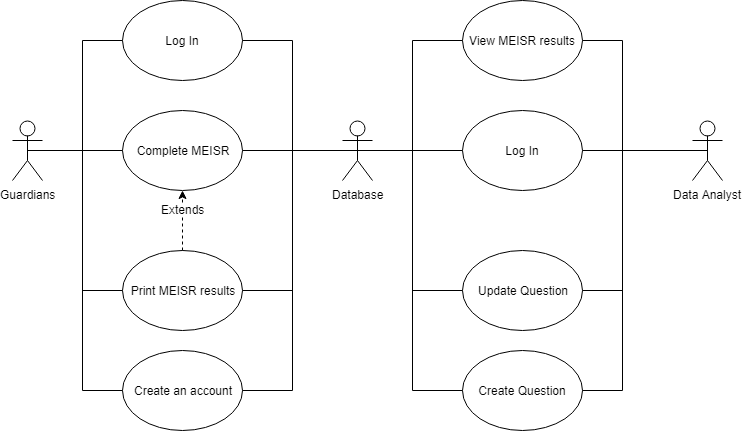
\includegraphics[width=0.7\textwidth]{images/Use_Case_Diagram.png}
  \caption{MEISR Use Case Diagram}
  \label{fig:useCase}
\end{figure}

Figure \ref{fig:useCase} shows three actors who will be interacting with out application. The first and most frequent actor will be the Guardians, or the people who fill out the survey about their children. The Guardian will have the options to Create and Account, Login, Complete MEISR, and Print MEISR Results. The second actor will be the Data Analyst who will query our back-end database to find trends or analyze results. The options available to him will be: Login, View MEISR Results, Update Question, and Create Question.

\section{UML Activity Diagrams}

\subsection{Create Account Activity Diagram}

\begin{figure}[h]
  \centering
  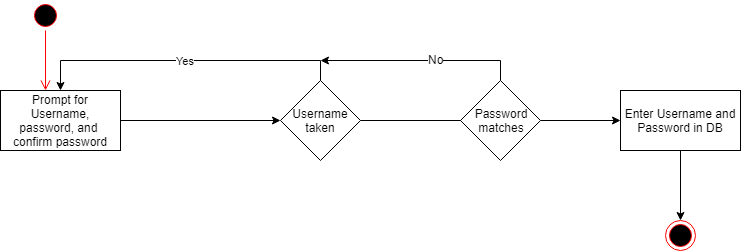
\includegraphics[width=0.7\textwidth]{images/Create_Account_Activity_Diagram.png}
  \caption{Create Account Activity Diagram}
  \label{fig:createAccount}
\end{figure}

Figure \ref{fig:createAccount} shows the process of creating an account. The user is prompted to enter a user name and password then confirm the password. The Database is queried to see if the user name is taken. If user name is free check that the password matches the confirm password. If both conditions are met enter the user name and password combination in the database. Otherwise prompt again.

\subsection{Log In Activity Diagram}

\begin{figure}[h]
  \centering
  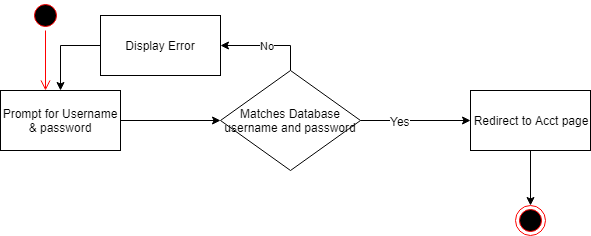
\includegraphics[width=0.7\textwidth]{images/Log_In_Activity_Diagram.png}
  \caption{Log In Activity Diagram}
  \label{fig:logIn}
\end{figure}

Figure \ref{fig:logIn} shows the process of logging in. First, prompt for user name and password. If the user name password combination matches one found in the database redirect to the account page. Otherwise display an error and redirect to the login prompt.

\subsection{Create Question Activity Diagram}

\begin{figure}[h]
  \centering
  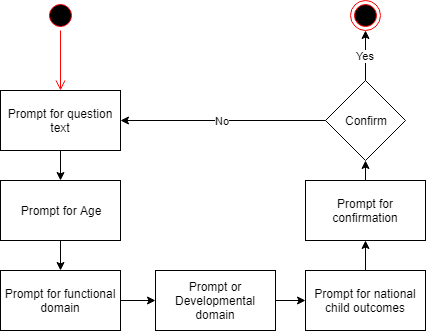
\includegraphics[width=0.7\textwidth]{images/Create_Question_Activity_Diagram.png}
  \caption{Create Question Activity Diagram}
  \label{fig:createQuestion}
\end{figure}

Figure \ref{fig:createQuestion} shows the process of creating a new MEISR question. The process begins by prompting for all necessary question fields (text, age, functional domain, etc.) then ask for confirmation after all information has been entered. If confirmation is given, add to the database. Otherwise redirect to the new question prompts.

\subsection{Update Question Activity Diagram}

\begin{figure}[h]
  \centering
  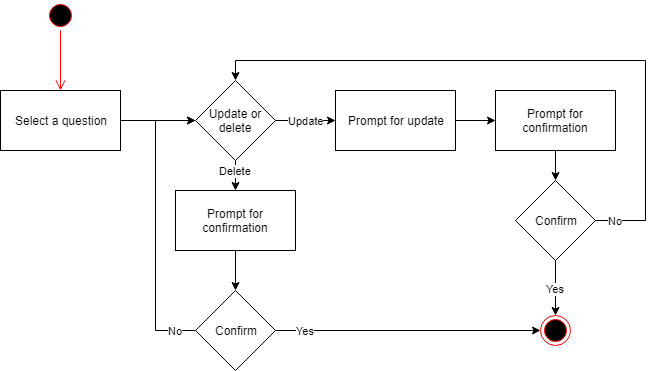
\includegraphics[width=0.7\textwidth]{images/Update_Question_Activity_Diagram.png}
  \caption{Update Question Activity Diagram}
  \label{fig:updateQuestion}
\end{figure}

Figure \ref{fig:updateQuestion} shows the process of updating a question. This process also includes deletion. After selecting a question, choose to update or delete the question. If delete, prompt for confirmation. If update, display all question fields and prompt for update then prompt for confirmation. If confirmed update the database otherwise redirect to update question prompts.

\subsection{Complete MEISR Activity Diagram}

\begin{figure}[h]
  \centering
  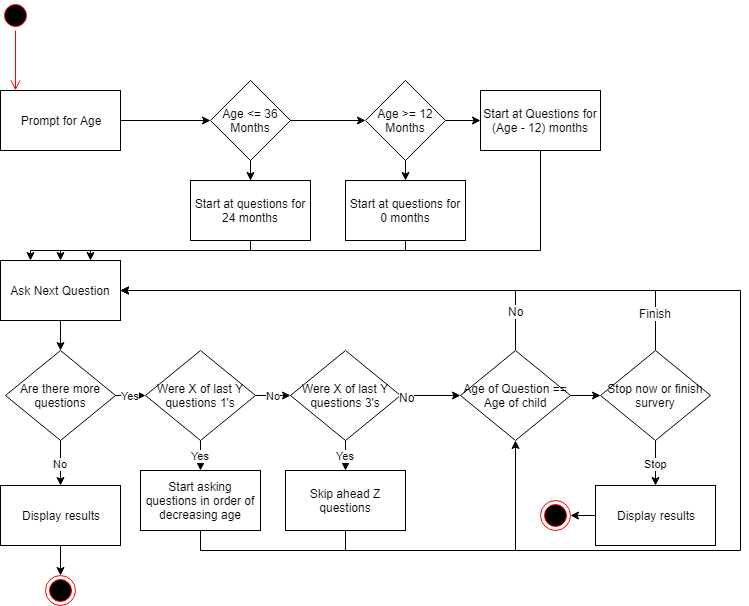
\includegraphics[width=0.7\textwidth]{images/Complete_MEISR_Activity_Diagram.png}
  \caption{Complete MEISR Activity Diagram}
  \label{fig:completeMEISR}
\end{figure}

Figure \ref{fig:completeMEISR} shows the process of completing the MEISR survery. Begin with a prompt for the child's age to determine at what age to start the questions. The questions will skip ahead or move back depending on the answers to previous questions. The questions end when there are no more questions or the parent reaches the child's age and chooses to stop rather than complete the remaining questions.

\subsection{View MEISR Results Activity Diagram}

\begin{figure}[h]
  \centering
  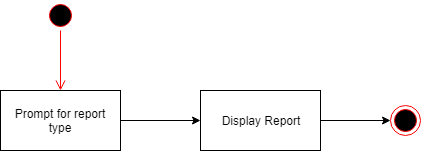
\includegraphics[width=0.7\textwidth]{images/View_MEISR_Results_Activity_Diagram.png}
  \caption{View MEISR Results Activity Diagram}
  \label{fig:viewMEISRResults}
\end{figure}
  
  Figure \ref{fig:viewMEISRResults} shows the process of displaying results for a completed MEISR survey. The user will select a report type from a selection of pre\-generated reports, and the report will display.
  
\section{UML High Level Class Diagram}

\begin{figure}[h]
  \centering
  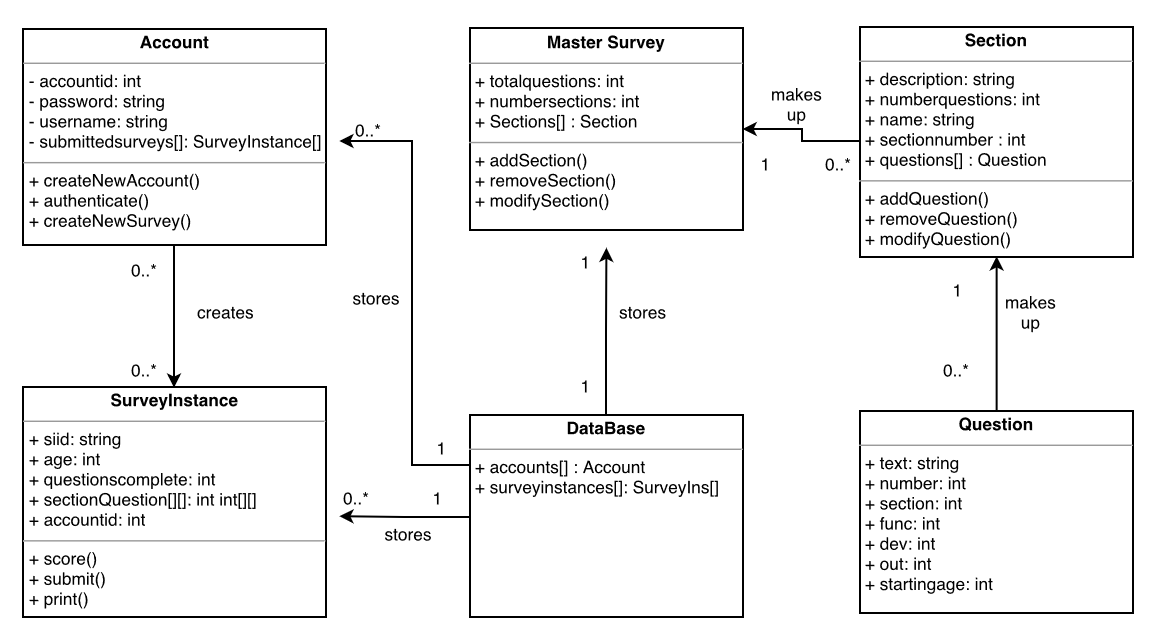
\includegraphics[width=0.7\textwidth]{images/HighLevelClassDiagramCS495.png}
  \caption{UML High Level Class Diagram}
  \label{fig:classDiagram}
\end{figure}

The classes we have proposed revolved around 3 main areas shown in figure \ref{fig:classDiagram}. First there is the Master Survey Class that contains the information about the current MEISR survey. If the current MEISR needs to be updated then the Master Survey Class is responsible for containing/changing that information. Second is the Account and Survey Instance class. This are both objects which will be created and stored in the database by users. This data can then be accessed later by researchers and clients. Lastly, the third area is the database itself, which needs to store accounts, surveys, and the master list.


Account Class
	The account class is created by a user when he first starts the app. It contains basic information such as username and password. It also contains a unique identification number, and all SurveyInstance objects created by this particular user in an Array.

SurveyInstance:
	An object of this class is created when the user starts a new MEISR survey. This class contains information such as the age of the child, how many questions have been completed, and it keeps track of the answers to that particular survey.

Question Class:
	This class contains the information needed to make a question such as text, number, description, ect. A question object is created and then added to an array of question objects in the section class.

Section Class:
	This class contains the information needed to make a section such as, section title, description, number, and all the questions contained in that section.

Master Survey:
	This class contains the information about the most up to date version of the MEISR, such as number of questions, number of sections, and an array of section objects, which contain the questions.

DataBase Class:
	This is not necessarily a class we will code, but it represents the entity of the database and how it interacts with our proposed system. We think we implement an SQL database as the information we need to store is mostly uniform. We also think that the SQL database will scale better with large tables versus querying large numbers of documents in a noSQL database.

\chapter{Design Diagrams}

\section{Detailed Class Diagram}

\begin{figure}[H]
  \centering
  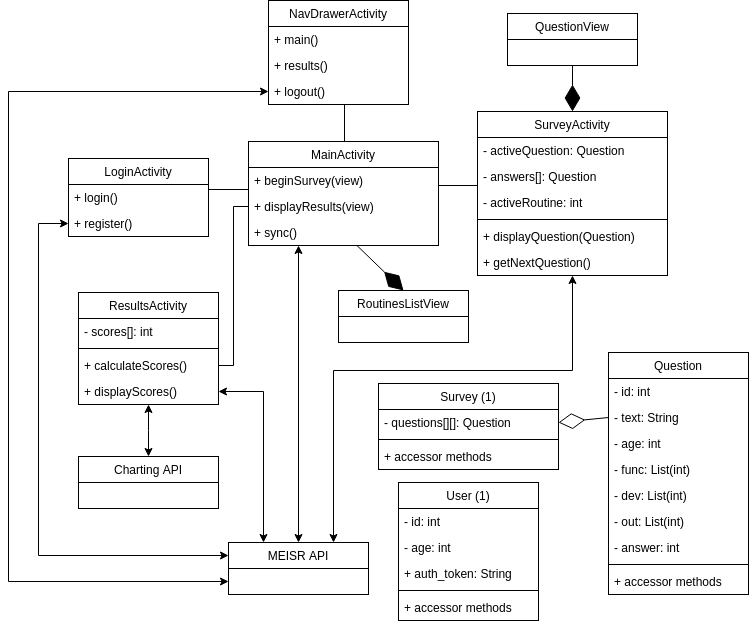
\includegraphics[width=0.7\textwidth]{images/design_class_dia.png}
  \caption{Detailed Class Diagram}
  \label{fig:detClassDiagram}
\end{figure}

Figure ~\ref{fig:detClassDiagram} shows the low-level class diagram for our Android application. To encapsulate the survey, we have a Survey class that contains a 2D array of Question objects. We are using a 2D array so that questions are organized by different routines. Each Question object has all of its relevant information along with an answer. There is also a User class so that we can handle authentication and store the age of the child. We want to use the singleton design pattern so that a single static instance of Survey and User can be accessed anywhere within the application. 

There will be five activities in our app, each of which communicate with the MEISR API. The MEISR API is simply a CRUD API for our backend/database. When the user opens the app, they will enter the LoginActivity which allows the user to login or register. After they are authenticated, the User class is populated with the user's id, age, and authentication token. Then, the user goes to a main screen where they can either start/continue the survey, or view their scores. This is also where the Survey class will be populated. The main screen will have a RoutineListView where clicking on a routine will begin the SurveyActivity starting at that routine. The SurveyActivity will show a QuestionView containing a text view of the question along with button views for their response. It will have a method to generate the views and another method to decide which question to ask next. There will also be a NavDrawerActivity so the user can quickly switch to different parts of the app, or logout of their account. Finally, in the ResultsActivity, the user can view their current scores as well as their previously saved scores. We will be using some sort of charting API to generate a graph of their scores over time.

\section{Database Schema}

\begin{figure}[H]
  \centering
  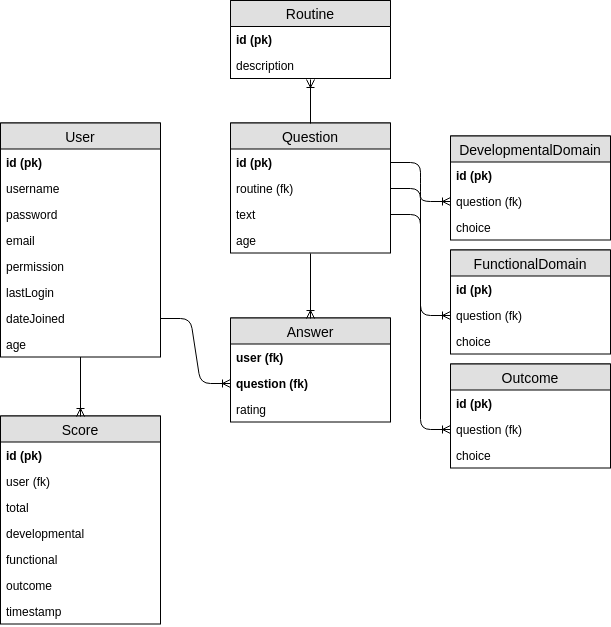
\includegraphics[width=0.7\textwidth]{images/db_schema.png}
  \caption{Database Schema}
  \label{fig:dbSchema}
\end{figure}

Figure ~\ref{fig:dbSchema} shows the schema of the database for our Django application. Django makes things very easy because we can define classes within our application, and the database is automatically created for us. This means that this diagram basically serves as a class diagram for our web application. Early on, we debated whether we should use a SQL or NoSQL database. While a survey could be intuitively stored in a document-store, we decided to go with a standard relational database. We wondered if scaling would ever be an issue with SQL, since answers for all users will be stored in the Answer table. However, our data models are fairly simple, and we don't believe our services will hit the point where a NoSQL database is needed. Also, Django only supports SQLite, MySQL, and PostgreSQL, which is the main reason we decided to go with a relational database. We are still undecided on whether we should use MySQL or PostgreSQL for our production environment. We will have to do some research on which will better serve EIEIO's needs.

The design of the database is fairly simple. First we have a table to store account information for each user. User can save scores and answers to survey questions, so we have a table for each. In the Answer table, we use a compound key of user id and question id so that each user only has one saved answer for each question. There is a single question table where Dr. McWilliam will be able to update or add new questions to the database. A question can be asked again in multiple routines, so we have a separate Routine table. Similarly, each question can have multiple developmental and functional domains as well as outcomes, so a table is needed for each. In order to implement all of our requirements, these tables should be sufficient. There are some other tables generated by default by Django and some of the packages we are using, but we have only included the tables from the classes we wrote ourselves.

\section{Sequence Diagrams}

\subsection{Create Question Sequence Diagram}
\begin{figure}[H]
  \centering
  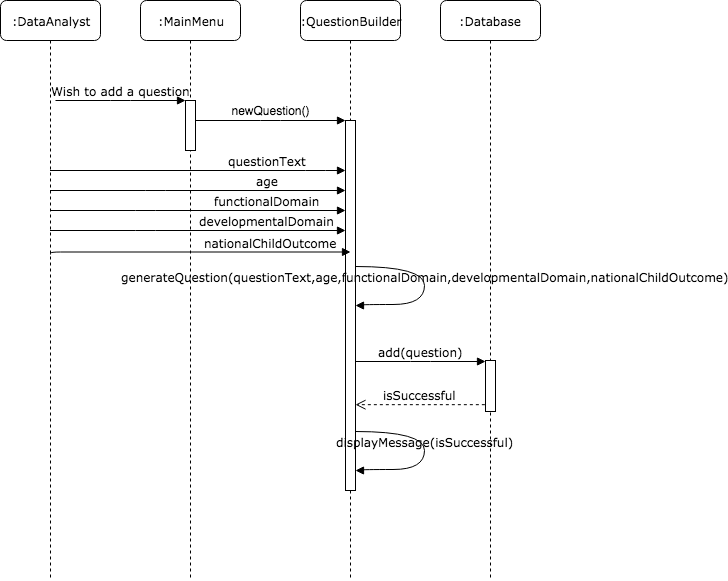
\includegraphics[width=0.7\textwidth]{images/CreateQuestionSequenceDiagram.png}
  \caption{Create Question Sequence Diagram}
  \label{fig:createQuestionSD}
\end{figure}

	Figure \ref{fig:createQuestionSD} shows the process for creating new MEISR questions to be displayed when taking the MEISR survey. This is only available to the data analyst from the web portal. The process begins with the data analyst's intent to create a new question. The data analyst selects the option from the main menu to add a question. The main menu will then redirect to the question builder where the data analyst must enter all of the required information for creating a question including the text, age, functional domain, developmental domain, and national child outcomes. The question builder will then generate a question from the provided information which is sent to the database. The database will return whether the question was successfully added and the question builder will then display a message indicating that the question was successfully added or display the error which prevented the question from being added.

\subsection{Update Question Sequence Diagram}
\begin{figure}[H]
  \centering
  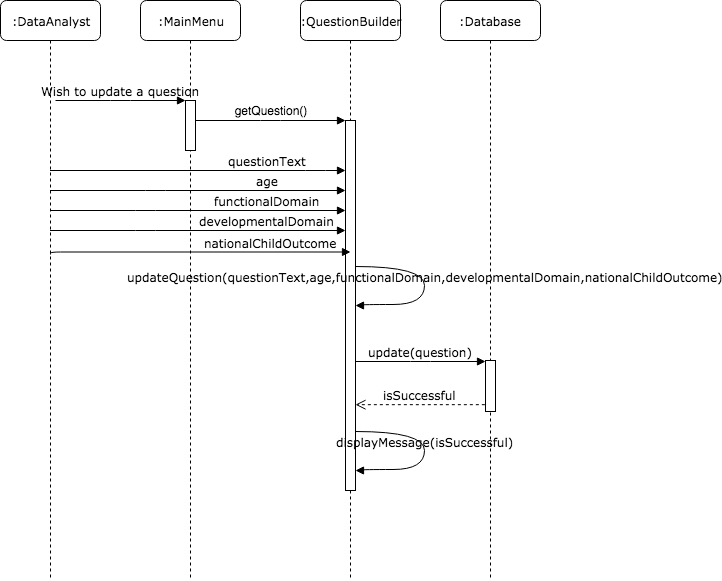
\includegraphics[width=0.7\textwidth]{images/UpdateQuestionSequenceDiagram.png}
  \caption{Update Question Sequence Diagram}
  \label{fig:updateQuestionSD}
\end{figure}

	Figure \ref{fig:updateQuestionSD} shows the process for updating an existing question within the MEISR survey. This is only available to the data analyst from the web portal. The process begins with the data analyst's intent to update a question. The data analyst selects a question to update which is then displayed by the question builder. The data analyst can update any of the fields of the question. The question builder will then update the question to reflect those changes and send the rebuilt question to the database.  The database will return whether the question was successfully updated and the question builder will then display a message indicating that the question was successfully updated or display the error which prevented the question from being updated.

\subsection{Delete Question Sequence Diagram}
\begin{figure}[H]
  \centering
  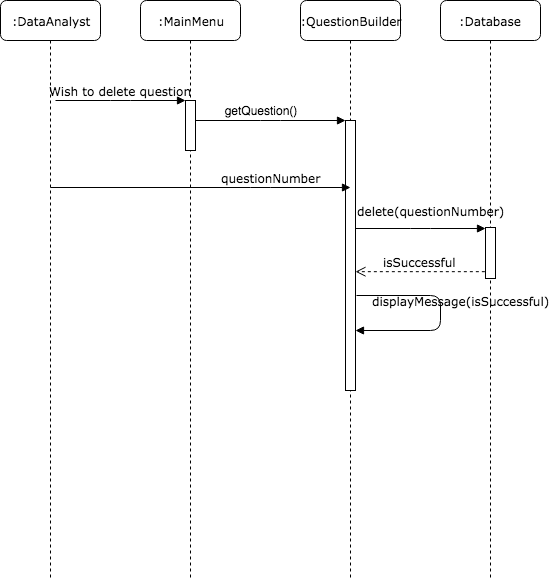
\includegraphics[width=0.7\textwidth]{images/DeleteQuestionSequenceDiagram.png}
  \caption{Delete Question Sequence Diagram}
  \label{fig:deleteQuestionSD}
\end{figure}

	Figure \ref{fig:deleteQuestionSD} shows the process for deleting an existing question within the MEISR survey. This is only available to the data analyst from the web portal. The process begins with the data analyst's intent to delete a question. The data analyst selects a question to be deleted based on question number. The database will delete the question with the selected question number, then whether the question was successfully deleted. The question builder will then display a message indicating that the question was successfully deleted or display the error which prevented the question from being deleted.

\subsection{Create Account Sequence Diagram}
\begin{figure}[H]
  \centering
  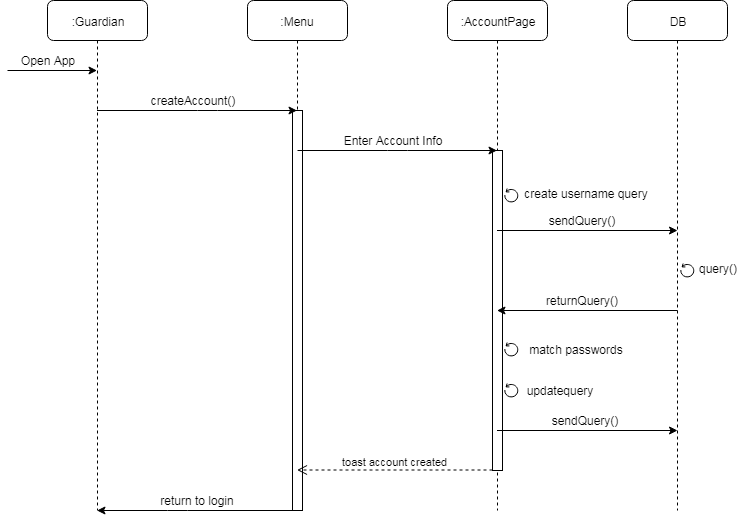
\includegraphics[width=0.7\textwidth]{images/createAccountSequenceDiagram.png}
  \caption{Create Account Sequence Diagram}
  \label{fig:createAccountSD}
\end{figure}

	Figure \ref{fig:createAccountSD} shows the process for creating an account when using the MEISR app. The process begins with a guardian who wishes to create an account. They select the create account option from the starting menu which directs them to the account page. The guardian must then enter all of the required account information. The account page will create a username query to ensure the username is unique indicated by the query's return value. The account page must then ensure that the password entered matches the password match field. If they match the account page can modify the query with all of the required account information and send this to the database. The account page will then return the guardian to the starting menu with a toast message indicating that the account has been created. This starting menu will then redirect the guardian to the log in page.

\subsection{Log In Sequence Diagram}
\begin{figure}[H]
  \centering
  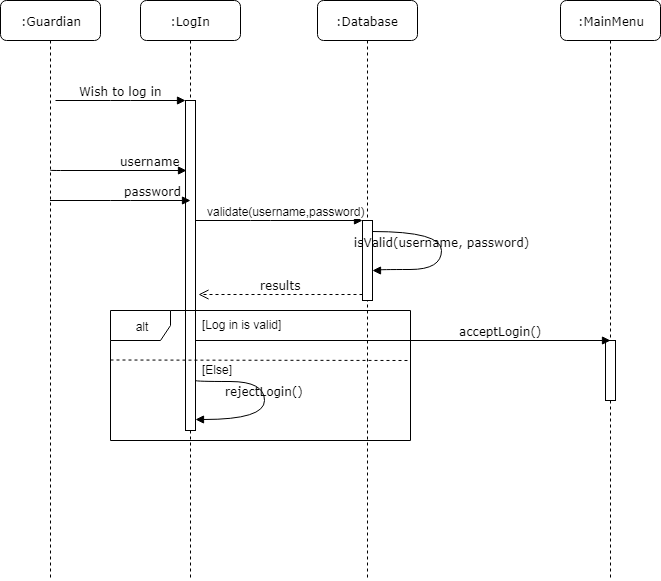
\includegraphics[width=0.7\textwidth]{images/LogInAppSequenceDiagram.png}
  \caption{App Log In Sequence Diagram}
  \label{fig:appLogInSD}
\end{figure}

\begin{figure}[H]
  \centering
  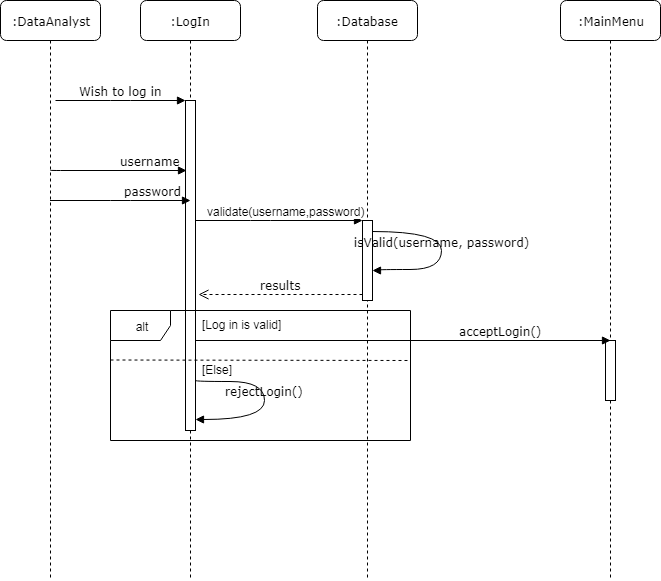
\includegraphics[width=0.7\textwidth]{images/LogInSequenceDiagram.png}
  \caption{Web Log In Sequence Diagram}
  \label{fig:webLogInSD}
\end{figure}

Figures  \ref{fig:appLogInSD} and \ref{fig:webLogInSD} show the process for logging in. These two diagrams are identical apart from the actor. Each begins with intent from the actor, guardian or data analyst, to log in. The actor must enter their username and password on the log in page. the log in page will then contact the database to verify the username and password combination. If the log in combination is valid,the actor will be redirected to the main page, otherwise the log in will be rejected and the actor will remain on the log in page with a message indicating the log in was unsuccessful.

\subsection{Complete MESIR Sequence Diagram}
\begin{figure}[H]
  \centering
  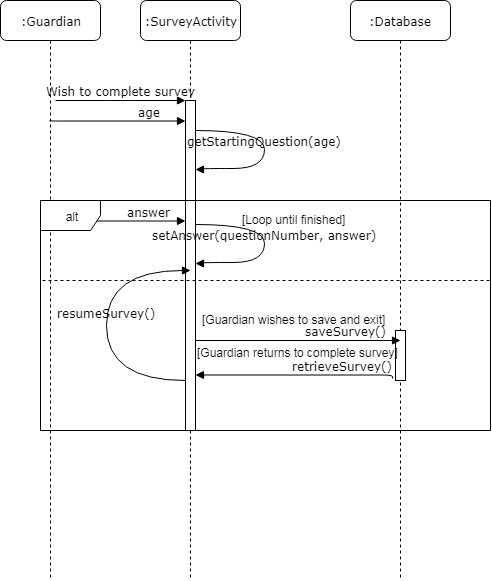
\includegraphics[width=0.7\textwidth]{images/CompleteMEISRSequenceDiagram.png}
  \caption{Complete MEISR Sequence Diagram}
  \label{fig:completeMEISRSD}
\end{figure}

	Figure \ref{fig:completeMEISRSD} shows the process for completing the MEISR survey. The process begins with the guardian who wishes to complete the survey. Before continuing the guardian must enter the age of the child about whom they are answering the questions. Using this age, the survey activity will determine which question the guardian will answer first. The guardian then has two paths which they can follow. The survey will continue to provide questions until the survey is complete setting the answer to each question when the guardian responds. However, the guardian can choose to save and exit at any time. If this happens the survey will be saved to the database in its current state. When the guardian returns to the survey the database will retrieve the survey and the guardian can resume answering questions. The survey activity will determine that the guardian is done when they have reached their child's age, when the survey has no further questions to answer, or when the answers to further questions can be assumed based on the pattern of previous answers. 

\subsection{View Results Sequence Diagram}
\begin{figure}[H]
  \centering
  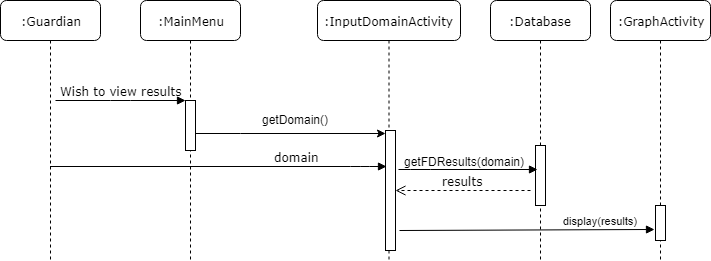
\includegraphics[width=0.7\textwidth]{images/ViewMEISRResultsSequenceDiagram.png}
  \caption{App View Results Sequence Diagram}
  \label{fig:appViewResultsSD}
\end{figure}

	The View MEISR Results sequence diagram, seen in figure \ref{fig:appViewResultsSD}, begins with a Guardian who wishes to view the results of their completed survey. The Guardian indicates this from a button from the Main Menu activity. From there, the Guardian then is taken to the Input Domain Activity where the guardian inputs their desired domain. This domain determines whether the displayed result will be an overall score, a specific domain, or outcome. Examples include: cognitive domain, developmental domain, or "postive social relations" outcome. Once the Guardian inputs their desired scoring domain, that domain is then sent to the database. The database returns the results back to the Input Domain Activity and then the results are put into the Graph Activity that will display the information for the Guardian.

\begin{figure}[H]
  \centering
  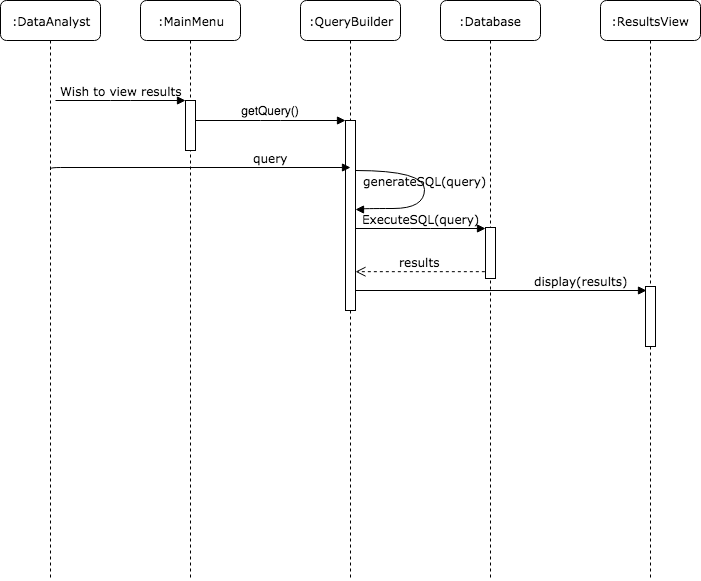
\includegraphics[width=0.7\textwidth]{images/ViewResultsSequenceDiagram.png}
  \caption{Web View Results Sequence Diagram}
  \label{fig:webViewResultsSD}
\end{figure}


	The data analyst also has the ability to view MEISR results. However, instead of viewing individual results, the data analyst will be able to view trends in the survey or in specific answers by querying the database. Figure \ref{fig:webViewResultsSD} shows the sequence diagram for this process, which is only available to the data analyst from the web portal. The process begins with data analyst's intent to view MEISR results. The data analysts selects this option from the main menu and is redirected to the query builder. The data analyst must then provide a query to the query builder. This will either be a manually constructed SQL query or a preconstructed query from a list of provided queries. The query builder will then construct this into a query which can be executed by the database and send it on. The database will return the results of this query to the query builder, which will send them to the results view to be displayed.

\begin{appendices}
%%%%%%%% GLOSSARY %%%%%%%%%
\chapter{Glossary}
\textbf{MEISR}: An acronym for “Measure of Engagement, Independence, and Social Relationships”, a survey created by Dr. McWilliam of EIEIO for the purpose of evaluating child development in the categories named as they grow.\\
\textbf{MEISR App}: The translation of the MEISR to an Android application with the purpose of providing a more powerful experience to users.\\
\textbf{Guardian}: A parent or primary caretaker of a child with a disability who is expected to be the primary operator of the app.\\
\textbf{Disability}: A documented case of some mental disability diagnosed by a psychological professional.\\
\textbf{Analyst}: A professional given access to the raw data collected by the MEISR app for the purpose of statistical analysis.\\
\textbf{Android}: A mobile operating system developed by Google based on the Linux operating system and other open source softwares.\\
\textbf{Android SDK}: a software development tool that provides APIs for creating Android apps using the Java programming language.\\
\textbf{API}: An acronym for “application programming interface”, a set of subroutines, protocols, and tools for building a software application.\\
%%%%%%%%%%%%%%%%%%%%%%
\end{appendices}





%%%%%%%%%%%%%%%%%%%%%%%%%%%%%%%%%%%%%%%%%%%%%%%%%%%%%%%%%%%%%%%%%%%%%%%%%%%%%%%%%
%% Source defintions
%%%%%%%%%%%%%%%%%%%%%%%%%%%%%%%%%%%%%%%%%%%%%%%%%%%%%%%%%%%%%%%%%%%%%%%%%%%%%%%%%
% When no use outcomment
%\bibliographystyle{alpha}

\renewcommand\bibname{References}
\bibliography{base/sources}


%%%%%%%%%%%%%%%%%%%%%%%%%%%%%%%%%%%%%%%%%%%%%%%%%%%%%%%%%%%%%%%%%%%%%%%%%%%%%%%%%
%% Inserting the appendix
%%%%%%%%%%%%%%%%%%%%%%%%%%%%%%%%%%%%%%%%%%%%%%%%%%%%%%%%%%%%%%%%%%%%%%%%%%%%%%%%%
% When no use outcomment
%\newpage
\appendix 
% Adds appendix as chapter to toc
\addcontentsline{toc}{chapter}{Appendix}


\chapter{First}


\chapter{Second}


\end{document}*/***********************************************************************8	
